GANs are generative models, similar to VAEs, but drop the assumption of optimizing the lower variational bound. Hence they often produce better results.\\
\b{Idea:} We want to sample from our training distribution, but there is now way to do this. Instead, we sample from a simple distribution, e.g. random noise, and learn the transformation to training distribution.\\

GANs consist of two networks: the Generator and the Discriminator. The Generator tries to fool the discriminator by generating real-looking images. The Discriminator then tries to distinguish between real and fake images. Both networks are trained jointly in an alternating fashion. We perform gradient \b{ascent} on the discriminator and gradient descent on the generator. The most important part during training is to have a good balance between Generator and Discriminator. It can easily happen that one outperforms/underperforms the other. After training, the generator can be used to generate new images.

\subsection{Diffusion Models}
Denoising diffusion models consist of two processes:
\begin{enumerate}
    \item Forward diffusion process gradually adds noise to input data by sampling from a Gaussian \f{T} times.
    \item Reverse denoising process generates output by denoising.
\end{enumerate}

The forward diffusion process is a Markov process that leads to the joint probability:
\cf{
    q(x_{1:T}|x_0) = \prod_{t=1}^{T}q(x_t|x_{t-1}) 
}
The schedule of the noise is designed such that \f{q(x_T|x_0)\approx\mathcal{N}(x_T; 0,1)}.\\

The denoising process starts by sampling \f{x_t\sim q(x_T)\approx\mathcal{N}(x_T;0,1)} and then iteratively sampling \f{x_{t-1}\sim q(x_{t-1}|x_t)}. Even though this is generally intractable, we can approximate this with a Gaussian if \f{\beta_t} is small enough. This means that we can learn the mean of a Gaussian to approximate \cf{q(x_{t-1}|x_t) \approx \mathcal{N}(x_{t-1};\mu_\theta(x_t,t),\sigma_t^2I),} where \f{\mu_\theta(x_t,t)} is the trainable network.

\begin{figure}[h!]
    \centering
    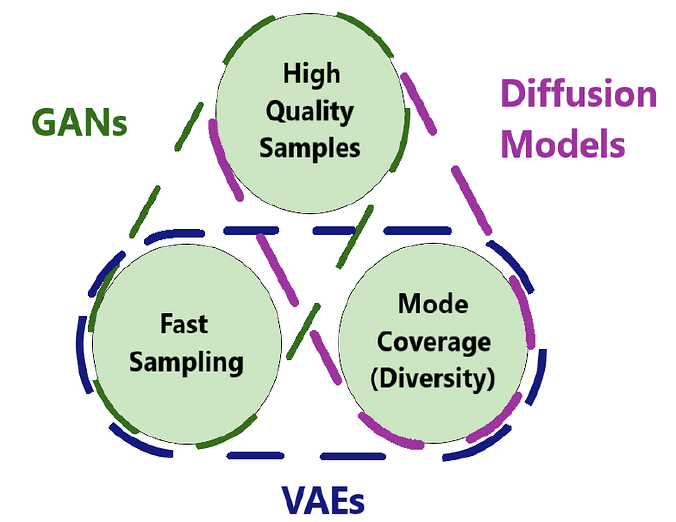
\includegraphics[width=0.4\textwidth]{gen.png}
\end{figure}